%-----------------------------------------------------------------------------------------------------------------------------------------------%
%	The MIT License (MIT)
%
%	Copyright (c) 2015 Jan Küster
%
%	Permission is hereby granted, free of charge, to any person obtaining a copy
%	of this software and associated documentation files (the "Software"), to deal
%	in the Software without restriction, including without limitation the rights
%	to use, copy, modify, merge, publish, distribute, sublicense, and/or sell
%	copies of the Software, and to permit persons to whom the Software is
%	furnished to do so, subject to the following conditions:
%	
%	THE SOFTWARE IS PROVIDED "AS IS", WITHOUT WARRANTY OF ANY KIND, EXPRESS OR
%	IMPLIED, INCLUDING BUT NOT LIMITED TO THE WARRANTIES OF MERCHANTABILITY,
%	FITNESS FOR A PARTICULAR PURPOSE AND NONINFRINGEMENT. IN NO EVENT SHALL THE
%	AUTHORS OR COPYRIGHT HOLDERS BE LIABLE FOR ANY CLAIM, DAMAGES OR OTHER
%	LIABILITY, WHETHER IN AN ACTION OF CONTRACT, TORT OR OTHERWISE, ARISING FROM,
%	OUT OF OR IN CONNECTION WITH THE SOFTWARE OR THE USE OR OTHER DEALINGS IN
%	THE SOFTWARE.
%	
%
%-----------------------------------------------------------------------------------------------------------------------------------------------%


%============================================================================%
%
%	DOCUMENT DEFINITION
%
%============================================================================%

%we use article class because we want to fully customize the page and dont use a cv template
\documentclass[10pt,A4]{article}	


%----------------------------------------------------------------------------------------
%	ENCODING
%----------------------------------------------------------------------------------------

%we use utf8 since we want to build from any machine
\usepackage[utf8]{inputenc}		

%----------------------------------------------------------------------------------------
%	LOGIC
%----------------------------------------------------------------------------------------

% provides \isempty test
\usepackage{xifthen}

%----------------------------------------------------------------------------------------
%	FONT
%----------------------------------------------------------------------------------------

% some tex-live fonts - choose your own

%\usepackage[defaultsans]{droidsans}
%\usepackage[default]{comfortaa}
%\usepackage{cmbright}
\usepackage[default]{raleway}
%\usepackage{fetamont}
%\usepackage[default]{gillius}
%\usepackage[light,math]{iwona}
%\usepackage[thin]{roboto} 

% set font default
\renewcommand*\familydefault{\sfdefault} 	
\usepackage[T1]{fontenc}
\usepackage{enumitem, hyperref}
\newcommand{\ts}{\textsuperscript}

% more font size definitions
\usepackage{moresize}		


%----------------------------------------------------------------------------------------
%	PAGE LAYOUT  DEFINITIONS
%----------------------------------------------------------------------------------------

%debug page outer frames
%\usepackage{showframe}			


%define page styles using geometry
\usepackage[a4paper]{geometry}		

% for example, change the margins to 2 inches all round
\geometry{top=1cm, bottom=0.8cm, left=1.5cm, right=1.5cm} 	

%use customized header
\usepackage{fancyhdr}				
\pagestyle{fancy}

%less space between header and content
%\setlength{\headheight}{-1.2cm}		


%customize entries left, center and right
\lhead{}
\chead{ 
	%\small{Sami Abdul Sater  $\cdot$ MA Ir. Informatique, BA. Sc. Physiques $\cdot$  Bruxelles, BEL  $\cdot$  \textcolor{sectcol}{\textbf{samiabdulsater@gmail.com}  $\cdot$ +32 487 35 53 25}
}
\rhead{}


%indentation is zero
\setlength{\parindent}{0mm}

%----------------------------------------------------------------------------------------
%	TABLE /ARRAY DEFINITIONS
%---------------------------------------------------------------------------------------- 

%for layouting tables
\usepackage{multicol}			
\usepackage{multirow}

%extended aligning of tabular cells
\usepackage{array}

\newcolumntype{x}[1]{%
>{\raggedleft\hspace{0pt}}p{#1}}%


%----------------------------------------------------------------------------------------
%	GRAPHICS DEFINITIONS
%---------------------------------------------------------------------------------------- 

%for header image
\usepackage{graphicx}

%for floating figures
\usepackage{wrapfig}
\usepackage{float}
%\floatstyle{boxed} 
%\restylefloat{figure}

%for drawing graphics		
\usepackage{tikz}				
\usetikzlibrary{shapes, backgrounds,mindmap, trees}


%----------------------------------------------------------------------------------------
%	Color DEFINITIONS
%---------------------------------------------------------------------------------------- 

\usepackage{color}
% Code couleur
\definecolor{LighterBlue}{rgb}{0.2,0.24,0.47}
\definecolor{DarkBlue}{rgb}{0.11,0.15,0.41}
\definecolor{NormalRed}{rgb}{0.9,0.2,0.16}

%accent color
\definecolor{OLDsectcol}{RGB}{50,0,0}
%\definecolor{sectcol}{rgb}{0.11,0.15,0.41}
\definecolor{bgcol}{rgb}{0.11,0.15,0.41}

%dark background color
\definecolor{OLDbgcol}{RGB}{110,110,110}
\definecolor{sectcol}{rgb}{0.11,0.15,0.41}
%\definecolor{bgcol}{rgb}{0.9,0.2,0.16}
%light background / accent color
\definecolor{softcol}{RGB}{225,225,225}

%arrow color
\definecolor{arrowcol}{rgb}{0,0.45,0.73}


%============================================================================%
%
%
%	DEFINITIONS
%
%
%============================================================================%

%----------------------------------------------------------------------------------------
% 	HEADER
%----------------------------------------------------------------------------------------

% remove top header line
\renewcommand{\headrulewidth}{0pt} 

%remove botttom header line
\renewcommand{\footrulewidth}{0pt}	  	

%remove pagenum
\renewcommand{\thepage}{}	

%remove section num		
\renewcommand{\thesection}{}			

%----------------------------------------------------------------------------------------
% 	ARROW GRAPHICS in Tikz
%----------------------------------------------------------------------------------------

% a six pointed arrow poiting to the left
\newcommand{\tzlarrow}{(0,0) -- (0.2,0) -- (0.3,0.2) -- (0.2,0.4) -- (0,0.4) -- (0.1,0.2) -- cycle;}	

% include the left arrow into a tikz picture
% param1: fill color
%
\newcommand{\larrow}[1]
{\begin{tikzpicture}[scale=0.58]
	 \filldraw[fill=#1!100,draw=#1!100!black]  \tzlarrow
 \end{tikzpicture}
}

% a six pointed arrow poiting to the right
\newcommand{\tzrarrow}{ (0,0.2) -- (0.1,0) -- (0.3,0) -- (0.2,0.2) -- (0.3,0.4) -- (0.1,0.4) -- cycle;}

% include the right arrow into a tikz picture
% param1: fill color
%
\newcommand{\rarrow}
{
\begin{tikzpicture}[scale=0.7]
	\filldraw[fill=sectcol!100,draw=sectcol!100!black] \tzrarrow
 \end{tikzpicture}
}



%----------------------------------------------------------------------------------------
%	custom sections
%----------------------------------------------------------------------------------------

% create a coloured box with arrow and title as cv section headline
% param 1: section title
%
\newcommand{\cvsection}[1]
{
\colorbox{sectcol}{\mystrut \makebox[1\linewidth][l]{
\larrow{white} \hspace{-6pt} \larrow{white} \hspace{-6pt} \larrow{white} \textcolor{white}{\textbf{#1}}\hspace{4pt}
}}\\
}

%create a coloured arrow with title as cv meta section section
% param 1: meta section title
%
\newcommand{\metasection}[2]
{
\begin{tabular*}{1\textwidth}{p{0.2\linewidth} p{0.75\linewidth}}
\larrow{bgcol}	\normalsize{\textcolor{sectcol}{#1}}&#2\\[12pt]
\end{tabular*}
}

%----------------------------------------------------------------------------------------
%	 CV EVENT
%----------------------------------------------------------------------------------------

% creates a stretched box as cv entry headline followed by two paragraphs about 
% the work you did
% param 1:	event time i.e. 2014 or 2011-2014 etc.
% param 2:	event name (what did you do?)
% param 3:	institution (where did you work / study)
% param 4:	what was your position
% param 5:	some words about your contributions
%
\newcommand{\cvevent}[5]
{
\vspace{8pt}
	\begin{tabular*}{1\textwidth}{p{2.7cm}  p{7.7cm} x{6.7cm}}
 \small{\textcolor{bgcol}{#1}}& \textbf{#2} & \vspace{2.5pt}\textcolor{sectcol}{#3}

	\end{tabular*}
\vspace{-12pt}
\textcolor{softcol}{\hrule}
\vspace{6pt}
	\begin{tabular*}{1\textwidth}{p{2.7cm} p{14.4cm}}
&		 \larrow{bgcol}  #4\\[3pt]
&		 \larrow{bgcol}  #5\\[6pt]
	\end{tabular*}

}

% creates a stretched box as 
\newcommand{\cveventmeta}[2]
{
	\mbox{\mystrut \hspace{87pt}\textit{#1}}\\
	#2
}

%----------------------------------------------------------------------------------------
% CUSTOM STRUT FOR EMPTY BOXES
%----------------------------------------- -----------------------------------------------
\newcommand{\mystrut}{\rule[-.3\baselineskip]{0pt}{\baselineskip}}

%----------------------------------------------------------------------------------------
% CUSTOM LOREM IPSUM
%----------------------------------------------------------------------------------------
\newcommand{\lorem}
{Lorem ipsum dolor sit amet, consectetur adipiscing elit. Donec a diam lectus.}



%============================================================================%
%
%
%
%	DOCUMENT CONTENT
%
%
%
%============================================================================%
\begin{document}


%use our custom fancy header definitions
\pagestyle{fancy}	


%---------------------------------------------------------------------------------------
%	TITLE HEADLINE
%----------------------------------------------------------------------------------------

% use this for multiple words like working titles etc.
%\hspace{-0.25\linewidth}\colorbox{bgcol}{\makebox[1.5\linewidth][c]{\hspace{46pt}\HUGE{\textcolor{white}{\textsc{Jan Küster}} } \textcolor{sectcol}{\rule[-1mm]{1mm}{0.9cm}} \parbox[b]{5cm}{   \large{ \textcolor{white}{{IT Consultant}}}\\
% \large{ \textcolor{white}{{Resume}}}}
%}}

% use this for single words, e.g. CV or RESUME etc.
\newgeometry{top=0.1cm, bottom=0.8cm, left=1.5cm, right=1.5cm} 	
\hspace{-0.25\linewidth}\colorbox{bgcol}{\makebox[1.5\linewidth][c]{\huge{\textcolor{white}{\textsc{
	Sami Abdul Sater
	}} } \textcolor{white}{\rule[-1mm]{1mm}{0.9cm}} \huge{\textcolor{white}{\textsc{
		Curriculum Vitae
		}} } }}



%----------------------------------------------------------------------------------------
%	HEADER IMAGE
%----------------------------------------------------------------------------------------

\vspace{2pt}
\cvsection{Summary}
\\[2pt]
\begin{minipage}{\textwidth}
	\centering
	\begin{minipage}{0.6\textwidth}
		I am a first year Master's student in computer engineering at Université Libre de Bruxelles, holding a bachelor degree in engineering sciences and also currently pursuing a bachelor in physical science. I have a great interest in the information technologies, cryptography, and a particular love toward physics. I am actively looking for an internship in the information technologies industry, both for my studies and to get more rounded by getting a first experience in the industry, after jobs and an internship in research at my university.\\[2pt]

		\metasection{Status:}{M.Eng. Computer Engineering, B.Sc. Physics, Student-assistant}
		\metasection{Fields:}{Cryptography, Databases, Data science, quantum information} 
	\end{minipage}
	\begin{minipage}{0.35\textwidth}
		\centering
		\begin{figure}[H]
			\centering
			\vspace{-0.5cm}
			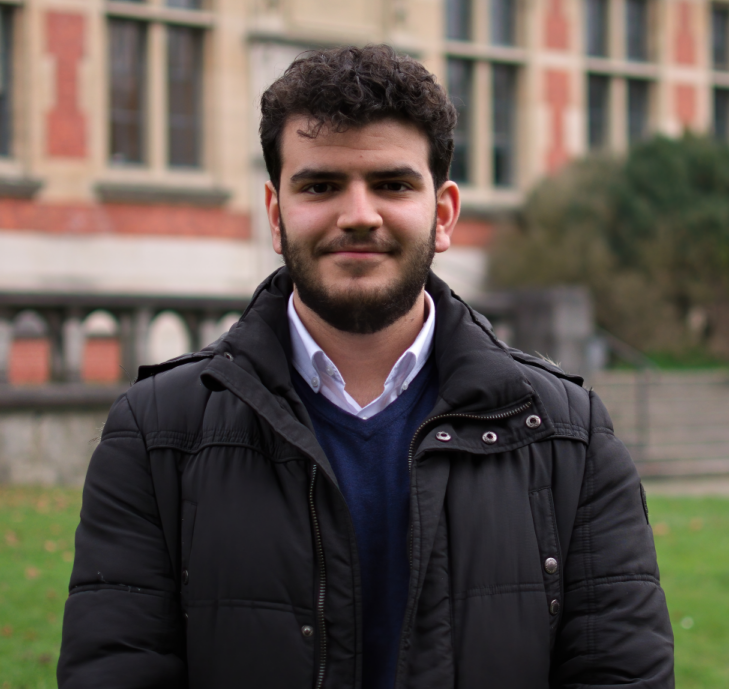
\includegraphics[width=0.7\linewidth]{myfoto_2.png}	%trimming relative to image size!
		\end{figure}
	\end{minipage}
\end{minipage}\\[3pt]

%---------------------------------------------------------------------------------------
%	QR CODE (optional)
%----------------------------------------------------------------------------------------
%\vspace{-136pt}
%\hspace{0.75\linewidth}
%\includegraphics[width=103pt]{qrcode}
%\normalsize
%\vspace{88pt}

%============================================================================%
%
%	CV SECTIONS AND EVENTS (MAIN CONTENT)
%
%============================================================================%

%---------------------------------------------------------------------------------------
%	EXPERIENCE
%----------------------------------------------------------------------------------------
\cvsection{Education}

\cvevent{2021 - Present}
{
	Master in Computer Engineering
}
{
	Université Libre de Bruxelles
}
{
	Relevant courses :  Quantum information and computation, Protocols, cryptanalysis and mathematical cryptology, Data warehouses, Advanced databases. 
	\\[-1pt]
	}
{
	My engineering curriculum is my main formation at University. It provides me theoretical concepts and useful tools to build a digital modelisation of the outside world, manipulate and protect information.
	\\[-2pt]
}

\cvevent{2020 - Present}{Bachelor in Physical Sciences}{Université Libre de Bruxelles}{
	Relevant courses : Quantum mechanics, Special relativity, Electromagnetism.
	\\[-1pt]
}{
	In parallel with my engineering curriculum, I am pursuing a degree in the Faculty of Sciences. It provides me with a more theoretical approach than the courses in my engineering curriculum. \\[2pt]
}

\cvevent{2018-2021}{Bachelor in engineering sciences (graduated)}{Université Libre de Bruxelles}{
	Minor in informatics. Relevant courses : Object oriented programmation, Operating systems, Operational resarch, Software engineering, Electronics, ...
	\\[-1pt]
}{
	Graduated with "\textit{Magna cum laude}" mention : GPA 3.3/4.\\[2pt]
	}
	\cvevent{2012-2018}{Higher education diploma (CESS)}{Athenée Robert Catteau}{
		"Mathematics and science" option
		}{
		Graduated with "\textit{Magna cum laude}" mention.\\[2pt]
	}

\cvsection{Academic projects}
\\[2pt]
\hspace{3pt}M. Eng. 
\begin{itemize}[label=\larrow{bgcol}]
	\item Secure chatting application.
	\item Compiler (fictif language).
	\item Monte-Carlo Tree Search for checkers game (Python)
	\item Implementing a new feature in \textit{PostgreSQL} (C) : join selectivity estimation for range types
\end{itemize}

\hspace{3pt}B. Sc. Physics
\begin{itemize}[label=\larrow{bgcol}]
	\item Exposition at Printemps des Sciences (ULB) : \textit{Acoustic Levitation}.
\end{itemize}

\newgeometry{top=1cm, bottom=0.8cm, left=1.5cm, right=1.5cm} 	
\hspace{3pt}B. Eng
\begin{itemize}[label=\larrow{bgcol}]
	\item 1\textsuperscript{st} year project : solar dryer for pepper seeds, to use for Kampot pepper, in Kampot, Cambodia. We've designed, dimensionned, built the prototype.
	\item 2\ts{nd} year project (biomedical-oriented) : motorisation of a 3D-printed hand to allow it to hold an egg without breaking it. Fishing lines and motors were used to mimic the tendons.
		
	\item Academic informatic projects : Scrabble in Python, Tower Defense in Java (JavaFX), Reversi (Minimax AI) in C++, project manager software in JavaFX.
\end{itemize} 



%---------------------------------------------------------------------------------------
%	EDUCATION SECTION
%--------------------------------------------------------------------------------------
\cvsection{Expérience}

\cvevent{02/2022-Present}{Co-author of a university syllabus}{ULB -- Faculté des Sciences}{
	In group of three students, we are currently writing course notes for the "Introduction to Quantum Mechanics" course in ULB, 2\ts{nd} year bachelor in physical sciences, under the supervision of the Professor (Serge Massar). We aim to make it the official course content.\\[1pt]
}{
	\href{https://www.ulb.be/fr/programme/phys-f203}{Link to the course page : PHYS-F203}
}

\cvevent{2019-Present}{Student representative}{ULB -- Ecole Polytechnique de Bruxelles}{
	I represent the students in my faculty in several ways: on the Faculty Council, on the "Filière informatique" Commission, on the Pedagogical, Teaching and Strategic Commissions.\\[1pt]
}{
	I have also been a student delegate since my second year at the University in order to organise contacts with the professors.
}

\cvevent{2021-Present}{Member of FabLAB ULB's student committee}{ULB -- FabLAB}{
	Manager of a student association from several faculties.\\[1pt]
}{The FabLab ULB is a complex within the digital network of FabLabs that finds its \textit{raison d'être} in a mixture of knowledge, know-how, collaboration, with the aim of acting on the world around us.}


\cvevent{07 - 08/2021}{Summer student intern (Applied Physics)}{ULB - Service de métrologie nucléaire}{
	I received a research initiation grant in order to discover the profession of researcher and to contribute to the work of a research department: the nuclear metrology department.	\\[1pt]
}{
	Within a research team, I was in charge of designing an optimisation algorithm for a machine used for proton therapy (IBA ProteusOne).
}

\cvevent{2020-2021}{IT Administrator}{ULB - Bureau Etudiant de Polytechnique}{
	Management, in duo, of the IT infrastructure of the student association of my faculty. Mainly: server management, website management (Wordpress), mailing lists.\\[1pt]
}{
	Development of some IT projects targeting the success of the Faculty's students: Alghoraires, an algorithm for optimal scheduling of oral exams according to individual student preferences, and a site providing an "Exam Question Bank".
}

\cvevent{2020-2022}{Student-assistant (x2)}{ULB - Ecole Polytechnique de Bruxelles}{
	In a group of 5 students, we worked on the improvement of the materials of the Analysis courses of the first two years of the Bachelor of Civil Engineering, taught by Pr. A. Delandtsheer; and with a student, for the Linear Algebra and Geometry course of Pr. J. Dohet-Eraly (MATH-H1001, MATH-H1002, MATH-H1003, MATH-H2000) \\[1pt]
}{
	Management of a document of several hundred pages in \LaTeX. Creation of figures (2D, 3D) using the TikZ package. Illustration of vector fields and 3D functions using the pgfplots package. \\[2pt]
}

\cvsection{Main skills}\\[2pt]
\metasection{Tools :}{\LaTeX, Python, Java, SQL, C++, Linux (Arch, Ubuntu), Office suite.}
\metasection{Technologies :}{Databases, Data visualization, Genetic algorithms.}
\metasection{Qualities :}{
	curious, efficient, hardworking, passionate, careful, organised.
}

\cvsection{Personal}\\[2pt]
\metasection{Hobbies :}{Boxing, soccer, reading, programming.}
\metasection{Languages :}{French (mother tongue), English (professional use), Dutch (basic knowledge), Arabic (basic knowledge).}
%-------------------------------------------------------------------------------------------------
%	ARTIFICIAL FOOTER (fancy footer cannot exceed linewidth) 
%--------------------------------------------------------------------------------------------------

% \null
% \vspace*{\fill}
% \hspace{-0.25\linewidth}\colorbox{bgcol}{\makebox[1.5\linewidth][c]{\mystrut \small \textcolor{white}{\href{https://www.linkedin.com/in/sami-abdul-sater-867469185/}{linkedin.com/in/sami-abdul-sater/}} $\cdot$ \textcolor{white}{
% 	\href{https://www.github.com/jemappellesami}{github.com/jemappellesami}
% }}}




%============================================================================%
%
%
%
%	DOCUMENT END
%
%
%
%============================================================================%
\end{document}
